\documentclass[a4paper]{article}

\usepackage{graphicx}


% content from this report was used as a basis for my presentation at WGISS-41
% titled: "Optimisation of Storage Structure to Enable Efficient File Access and Processing on Massive Time-series of EO Data"
% \title{Chunksize and Compression Level Testing}
\title{Optimisation of Storage Structure to Enable Efficient File Access and\\ Processing on Massive Time-series of EO Data}
\date{November 30 2015}
\author{Josh Sixsmith}

\begin{document}
  \pagenumbering{gobble}
  \maketitle
  \newpage
  \pagenumbering{arabic}

  \section{Introduction}

    \begin{flushleft}
    The HDF5 file format enables users to build highly tunable data access and storage solution tailored to meet their everyday needs and requirements. \par
    This report examines the comparison of differing chunksizes for both a 2D spatial domain (x \& y axis), as well as 3D (z axis) storage blocks, and at varying compression levels in relation to storing Earth Observation imagery.
    \end{flushleft}

  \section{method}

    \begin{flushleft}
    14 spatial cells, approximately 1.0 degrees by 1.0 degrees with a 25 metres pixel resolution, were selected because of their spatial position relative to the WRS2 Landsat grid. These cells contain varying amounts of data coverage, ranging from sparse (mostly null data) to complete valid data coverage.   \par
    Imagery acquired by Landsat 5 from the year 2008 was used due to SLC-OFF issues with Landsat 7. \par
    The spatial dimensions of each cell were 4000 by 4000 pixels, whereas the z-axis differed from cell to cell but within the range of 13 to 23 slices. \par
    The z-axis chunk sizes used were 5, 10 \& 20, and for each z-axis chunk size, each of the follwoing spatial chunks were applied:
    \end{flushleft}

    \begin{itemize}
      \item 50
      \item 75
      \item 100
      \item 150
      \item 200
      \item 300
      \item 400
    \end{itemize}

    \begin{flushleft}
    For each chunksize combination, a different compression filter from the following list was applied:
    \end{flushleft}

    \begin{itemize}
      \item GZip level 1
      \item GZip level 4
      \item GZip level 8
      \item LZF
    \end{itemize}

    \begin{flushleft}
    To add to the combinations, each compression filter was set with and without a shuffle filter in order to evaluate any additional compression gains that a shuffle filter may provide. \par
    The total number of combinations resulted in 2352 files, and for further comparison of read acces, raw uncompressed files were also generated.

    The following figure displays the area selected for the storge uints compression testing. Cells that interesected the geometries of Path 90 and Rows 84/85 from the WRS2 *descending* grid, were then used to form the data basis of this report. As one can see, the cell grid data layout results in sparse data as well as dense data, within a given cell, for a given acquisition date.
    \end{flushleft}

    \begin{figure}[h!]
      \centering
      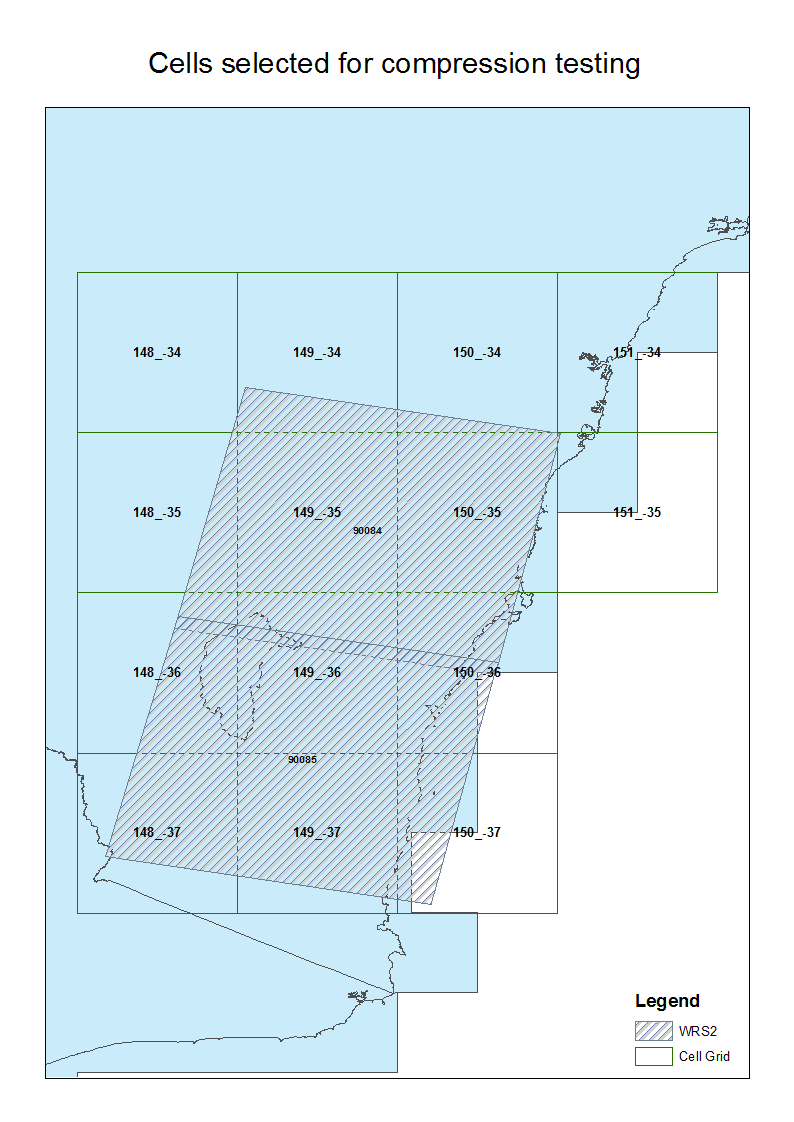
\includegraphics[scale=0.5]{storage-units-compression-testing-selected-area.png}

    % ![alt text](storage-units-compression-testing-selected-area.png)
    \end{figure}

  \newpage

  \section{Results}

    \begin{flushleft}
    The shuffle filter didn't have the desired affect reducing the filesize, most likely due to the variabiity of the data contained within a given chunk.  As such it was excluded early on in the comparative analysis. \par
    The conducted read test was simply to read all the data for a given \textit{compression xy chunk z chunk} setting for each cell. This was simply to emulate a workflow processing all data. \par
    It has already been noted in a previous report that processing data using a chunksize smaller than the storage chunksize can have significant impacts on an algorithmic workflow. \par
    With so many differing chunksizes, this was undesireable to test, and could result in highly skewed results.
    \end{flushleft}

    \subsection{Compression Ratios}

      Compression ratios of each cell, at varying spatial chunksizes.
    
      \begin{flushleft}
      There is slight variation in filesizes between cells, but this is expected due to the WRS2 swath locations, thereby depending on the acquisition date, some cells have partial data, while others have more complete coverage. \par
      For the data used in this comparison overview, it was observed that chunksizes not being an exact multiple of the array dimensions had a small but fairly negligible affect on overall filesize.
      \end{flushleft}

    % ![alt text](Compression-ratio-per-cell-z_chunk-5.png)
    % ![alt text](Compression-ratio-per-cell-z_chunk-10.png)
    % ![alt text](Compression-ratio-per-cell-z_chunk-20.png)
      \begin{figure}[h!]
        \centering
        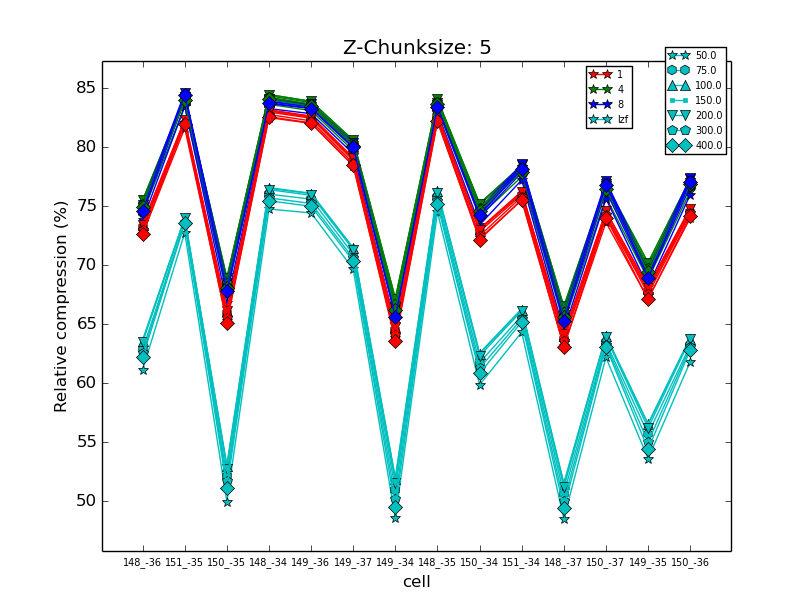
\includegraphics[scale=0.5]{Compression-ratio-per-cell-z_chunk-5.png}
      \end{figure}
    
      \begin{figure}[h!]
        \centering
        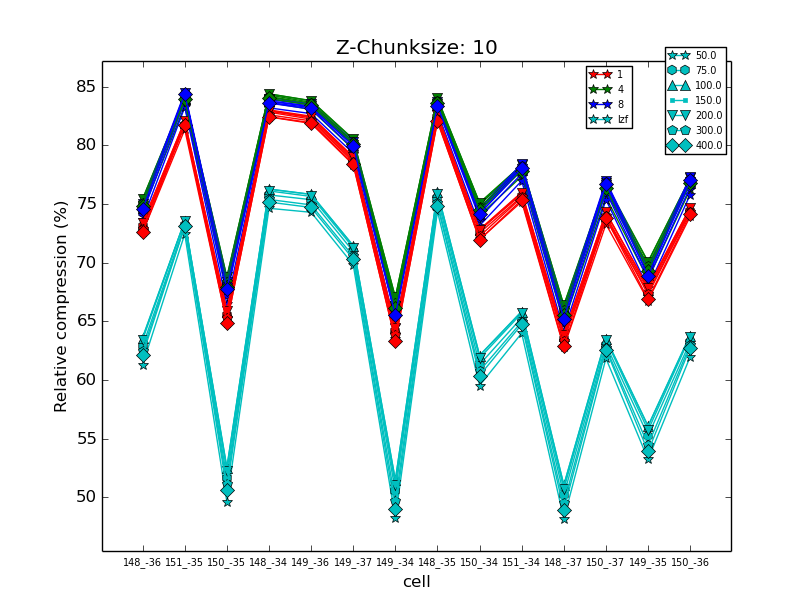
\includegraphics[scale=0.5]{Compression-ratio-per-cell-z_chunk-10.png}
      \end{figure}
    
      \begin{figure}[h!]
        \centering
        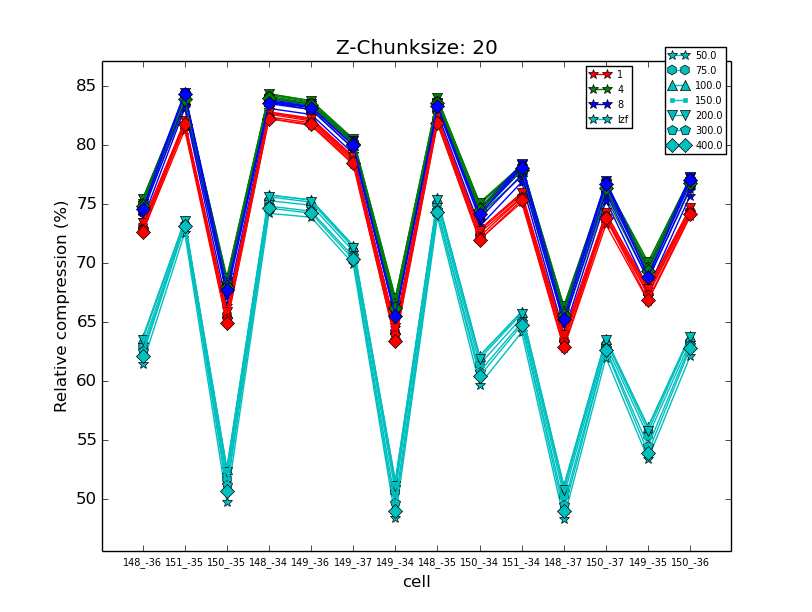
\includegraphics[scale=0.5]{Compression-ratio-per-cell-z_chunk-20.png}
      \end{figure}
    
    \newpage

    \subsection{Read Times}

      Total read time vs compression ratio
    
      \begin{flushleft}
      It is interesting to note that while the filesize decreased with an increasing spatial chunksize, at the 300 \& 400
      chunksize, the filesize increased. This trend hasn't been investigated further, but one could make the assumption
      that due to the nature of the data, that the spatial variability has some influence on the overall compression.
      The hypthesis is that less homogenous data compresses poorly compared to data of a more homogenous state.
      
      For a further comparitive investigation, raw uncompressed files were also generated. The raw files were written
      using a natural scanline blocksize. In terms of total read time, only some files compressed using the LZF
      algorithm outperformed the raw binary files.
      \end{flushleft}
      
      % ![alt text](Compression-ratio-vs-Read-time-z_chunk-5.png)
      % ![alt text](Compression-ratio-vs-Read-time-z_chunk-10.png)
      % ![alt text](Compression-ratio-vs-Read-time-z_chunk-20.png)
      \begin{figure}[h!]
        \centering
        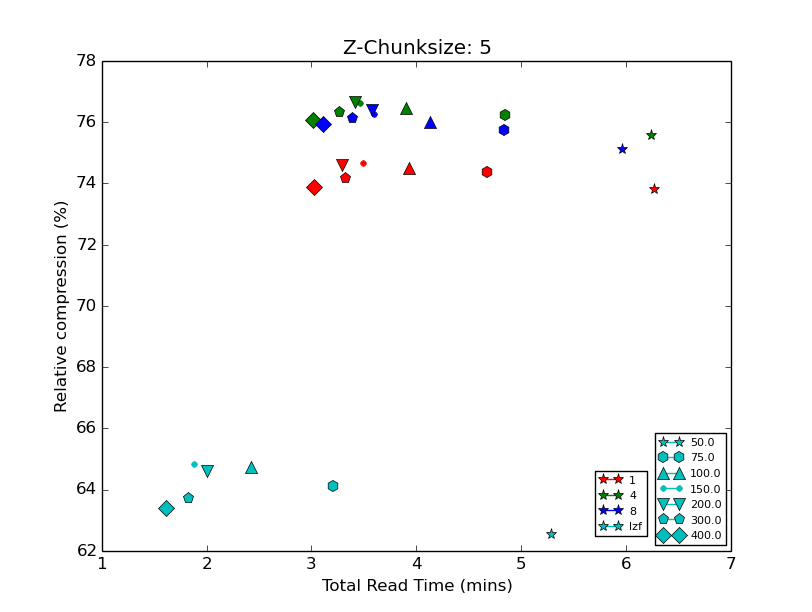
\includegraphics[scale=0.5]{Compression-ratio-vs-Read-time-z_chunk-5.png}
      \end{figure}
    
      \begin{figure}[h!]
        \centering
        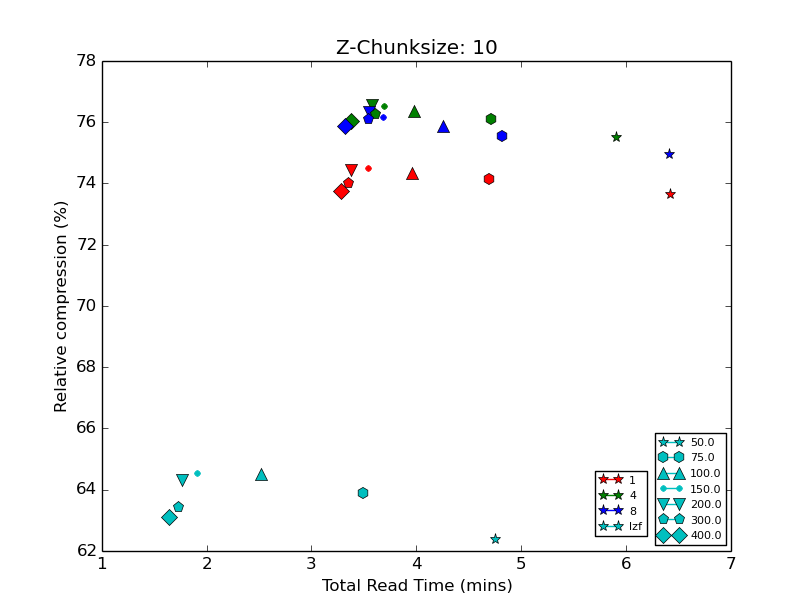
\includegraphics[scale=0.5]{Compression-ratio-vs-Read-time-z_chunk-10.png}
      \end{figure}
    
      \begin{figure}[h!]
        \centering
        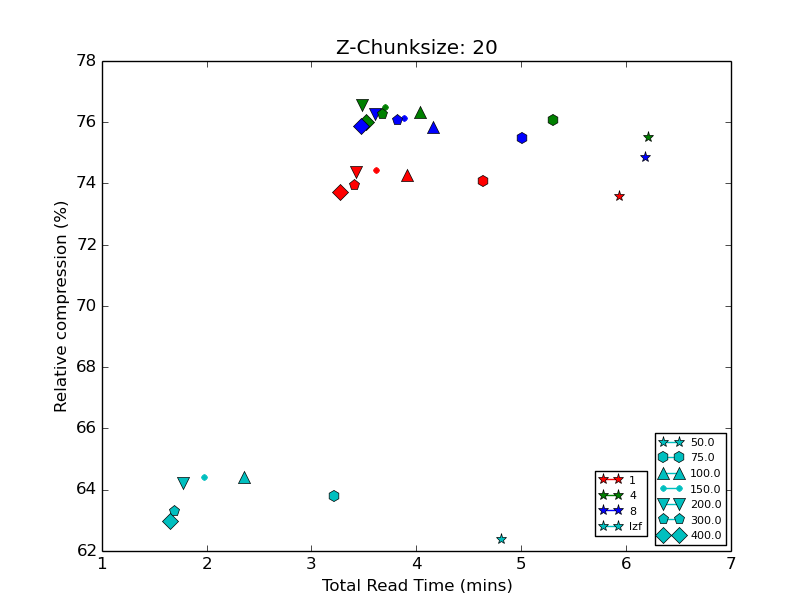
\includegraphics[scale=0.5]{Compression-ratio-vs-Read-time-z_chunk-20.png}
      \end{figure}
    
  \newpage

      % ![alt text](Compression-ratio-vs-Read-time-z_chunk-5_raw.png)
      % ![alt text](Compression-ratio-vs-Read-time-z_chunk-10_raw.png)
      % ![alt text](Compression-ratio-vs-Read-time-z_chunk-20_raw.png)
      \begin{figure}[h!]
        \centering
        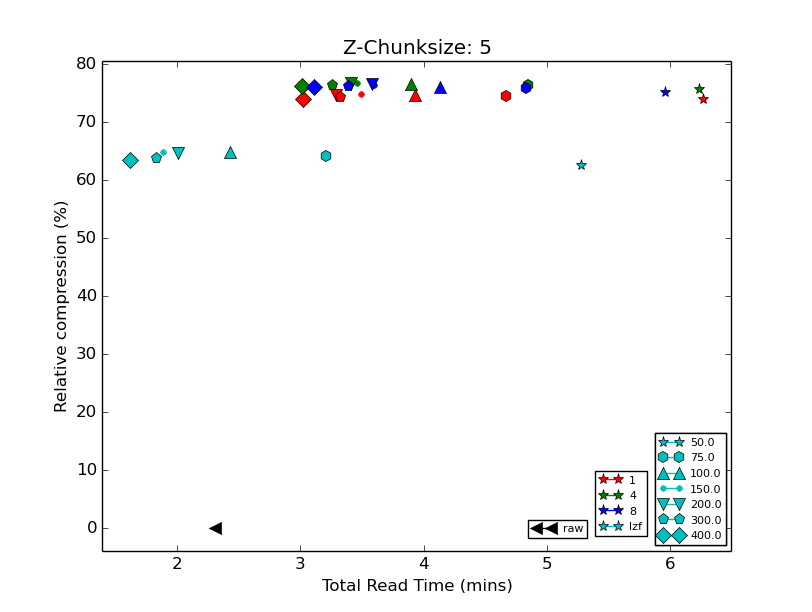
\includegraphics[scale=0.5]{Compression-ratio-vs-Read-time-z_chunk-5_raw.png}
      \end{figure}
    
      \begin{figure}[h!]
        \centering
        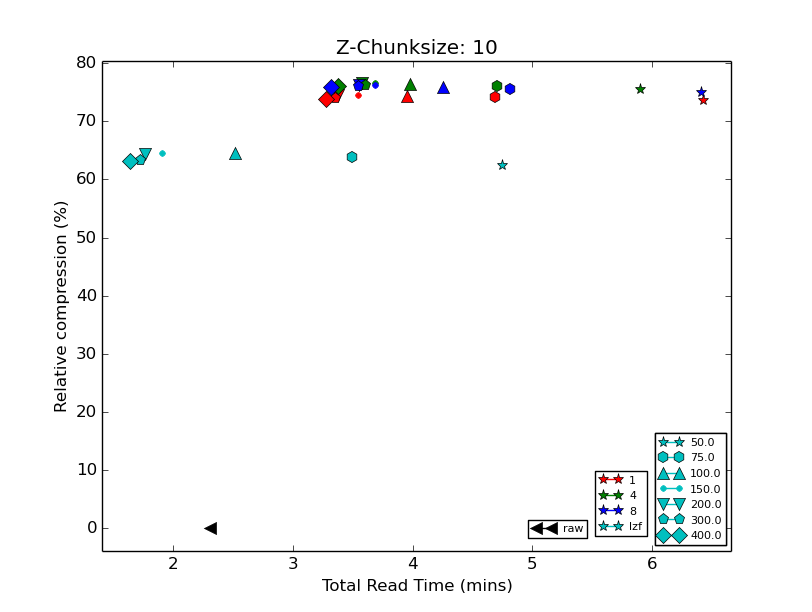
\includegraphics[scale=0.5]{Compression-ratio-vs-Read-time-z_chunk-10_raw.png}
      \end{figure}
    
      \begin{figure}[h!]
        \centering
        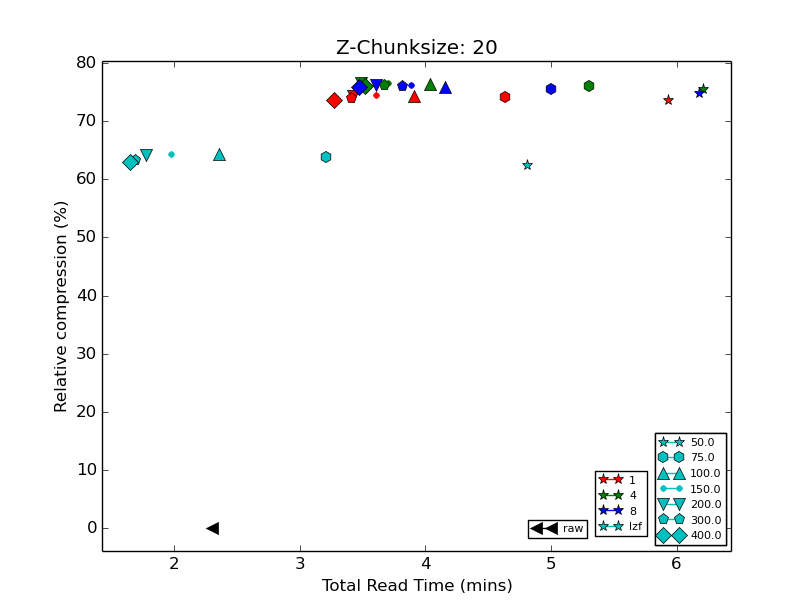
\includegraphics[scale=0.5]{Compression-ratio-vs-Read-time-z_chunk-20_raw.png}
      \end{figure}

  \newpage

  \section{Summary}

    \begin{flushleft}
    Overall, the spatial blocksize of 200 performed well alround for each compression setting, and \textit{z} chunksize. This is not to say that a spatial blocksize of 200 will be performant for all workflows. As previously noted reading a block smaller than 200 will incurr performance penalties if the goal is to process the entire spatial dimension. This will also be true for any blocksize. \par
    The filesizes for a given \textit{spatial} chunksize and compression filter differed slightly between the thre \textit{z} axis chunksizes. A \textit{z} chunksize of 5 tended to have better better compression ratios, potentially due to more complete chunks being written to disk as opposed to partial chunks. However, the total read times tended to be longer. \par
    As for the compression algorithms, in terms of raw speed, the LZF algorithm significantly performed better at all \textit{spatial} and \textit{z} chunksize than the other compression settings. The compression ratios were slightly lower in the range of 10-15\% than the GZip equivalents. \par
    The default setting of \textit{4} for the GZip algorithm, tended to get higher compression ratios than even the level \textit{8} GZip setting. In some instances GZip level \textit{4} also had better read times than levels \textit{1} or \textit{8}.
    \end{flushleft}
\end{document}
